\documentclass[12pt,a4paper]{article}
\usepackage[utf8]{inputenc}
\usepackage[english,russian]{babel}
\usepackage{indentfirst}
\usepackage{misccorr}
\usepackage{graphicx}
\usepackage{amssymb}
\usepackage{amsmath}

\begin{document}

\begin{center}
    \large
    Работа 1.2.5
    
    Сибгатуллин Булат, Б01-007
    
    \vspace{0.5cm}
    \textbf{Исследование вынужденной регулярной прецессии гироскопа}

\end{center}

\vspace{0.5cm}
\textbf{Цель работы:} исследовать вынужденную прецессию гироскопа; установить зависимость скорости вынужденной прецесси от величины момента сил, действующих на ось гироскопа;определить скорость вращения ротора гироскопа и сравнить ее со скоростью, рассчитанной по скорость прецесии.

\vspace{0.5cm}
\textbf{В работе используются:} гироскоп в кардановом подвесе, секундомер, набор грузов, отдельный ротор гироскопа, цилиндр известной массы, крутильный маятник, штангенциркуль, линейка.

Гироскопом принято называть тело, для которого, например,

\[I_z\omega_z \gg I_x \omega_x, \: I_y \omega_y,\]

где $I_x, I_e, I_z$ - главные моменты инерции, $\omega_x, \omega_y, \omega_z$ - компоненты вектоа уголовой скорости $\overrightarrow{\omega}$. Уравновешенным гироскопом называют гироскоп, у которого центр масс неподвижен.

Выясним, какие силы нужно приложить к гироскопу, чтобы изменить направление его оси. Пусть:

\[\omega_z = \omega_0, \quad \omega_x = 0, \quad \omega_y = 0.\]

\begin{equation}
L_{\Omega} \ll L_{\omega_0}.
\end{equation}

Здесь $\Omega$ -  угловая скорость такого вращения.

Выполнив вычисления получим:

\begin{equation}
\overrightarrow{M} = \overrightarrow{\Omega} \times \overrightarrow{L}
\end{equation}

Формула (2) справедлива, если выполнено условие (1). Под действием момента $\overrightarrow{M}$ внешних сил ось гироскопа медленно вращается вокруг оси \textit{y} с угловой скоростью $\Omega$. Такое движение называют регулярной прецессией гироскопа. Для гироскопа массой $m_{\textit{г}}$, у которого ось собственного вращения наклонена на угол $\alpha$ от вертикали, скорость прецессии, происходящей вокруг вертикальной оси под действием силы тяжести, равна

\begin{equation}
\Omega = \frac{M}{I_x \omega_0 \sin \alpha} = \frac{m_{\textit{г}} g l_{\textit{ц}} \sin \alpha}{I_z \omega_0 \sin \alpha} = \frac{m_{\textit{г}} g \l_{\textit{ц}}}{I_z \omega_0},
\end{equation}

где $l_{\textit{ц}}$ - расстояние от точки подвесадо центра масс гироскопа, т.е. скорость прецессии не зависит от угла $\alpha$.

Для изучения регулярной прецессии уравновешенного гироскопа к его оси подвешивают дополнительные грузы. Это смещает общий центр масс и создает момент сил тяжести, вызывающий прецессию. Скорость прецессии в этом случае равна

\begin{equation}
\Omega = \frac{mgl}{I_z \omega_0},
\end{equation}

где \textit{m} - масса груза, \textit{l} - расстояние от центра карданова подвеса до точки крепления груза на оси гироскопа (рис. 1).

\begin{figure}[h!]
\centering
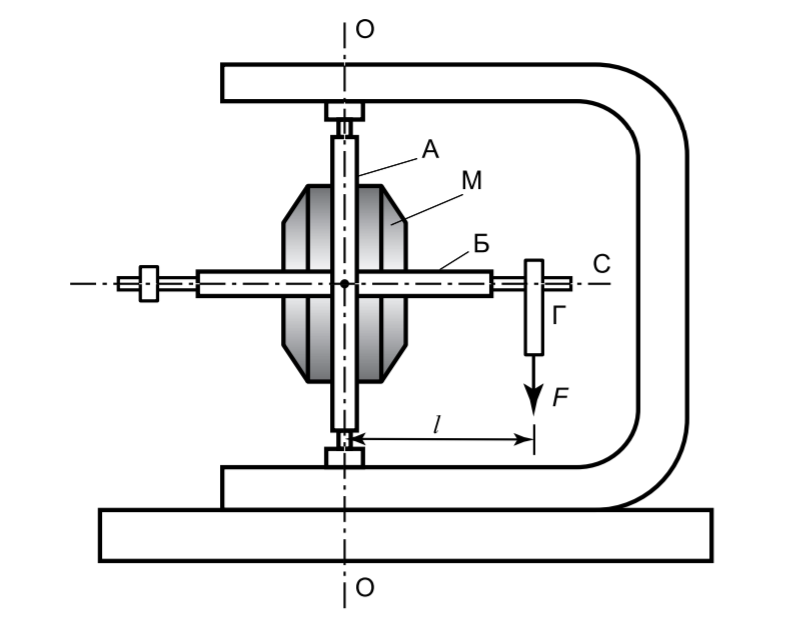
\includegraphics[scale=0.7]{Experimental_setup.png}
\caption{Схема экспериментальной установки}
\label{fig:Experimental setup}
\end{figure}

Измерение скорости прецессии гироскопа позволяет вычислить скорость вращения его ротора. Расчет производится по формуле (4). Момент инерции ротора относительно оси симметрии $I_0$ измеряется по крутильным колебаниям точной копии ротора, подвешиваемой вдоль оси симметрии на жесткой проволоке. Период крутильных колебаний $T_0$ зависит от момента инерции $I_0$ и модуля кручения проволоки \textit{f}:

\begin{equation}
T_0 = 2\pi \sqrt{\frac{I_0}{f}}.
\end{equation} 

Чтобы исключить модуль кручения проволоки, вместо ротора гироскопа к той же проволоке подвешивают цилиндр правильной формы с известными размерами и массой, для которого можно легко вычислить момент инерции $I_{\textit{ц}}$. Для определения момента инерции ротора имеем

\begin{equation}
I_0 = I_{\textit{ц}} \frac{T_0^2}{T_{\textit{ц}}^2},
\end{equation}

здесь $T_{}\textit{ц}$ - период крутильных колебаний цилиндра.

Скорость вращения ротора гироскопа можно измерить и не прибегая к исследованию прецессии. У используемых в работе гироскопов статор имеет две обмотки, необходимые для быстрой раскрутки гироскопа. В данной работе одну обмотку используют для раскрутки гироскопа, а вторую - для измерения числа оборотов ротора.

\vspace{3cm}

Кратковременное воздействие на вращающийся гироскоп.

\begin{figure}[h!]
\centering
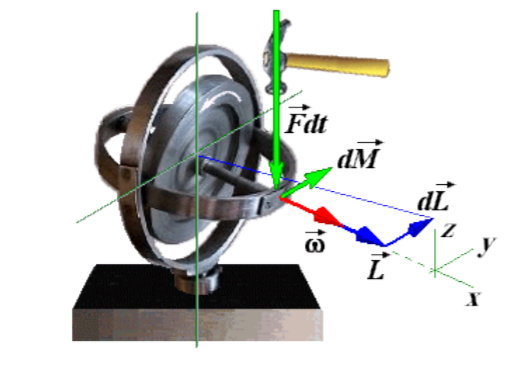
\includegraphics[scale=0.7]{kick_hyro.png}
\caption{Удар по гироскопу}
\label{fig:Kick hyro}
\end{figure}

Если сообщить гироскопу импульс $\overrightarrow{F}dt$, то создаваемый кратковременный момент внешних сил $d\overrightarrow{M}$ и приращение момента импульса $d\overrightarrow{L}$ перпендикулярны оси вращения и вектору $\overrightarrow{L}$

Поскольку гироскоп вращается очень быстро, а время ударного воздействия мало, то отношение $d\overrightarrow{L} / \overrightarrow{L}$ также очень мало и направление оси вращения не изменится.

В качестве примера можем рассмотреть номер 11.7  из задачника по физике.

\begin{figure}[h!]
\centering
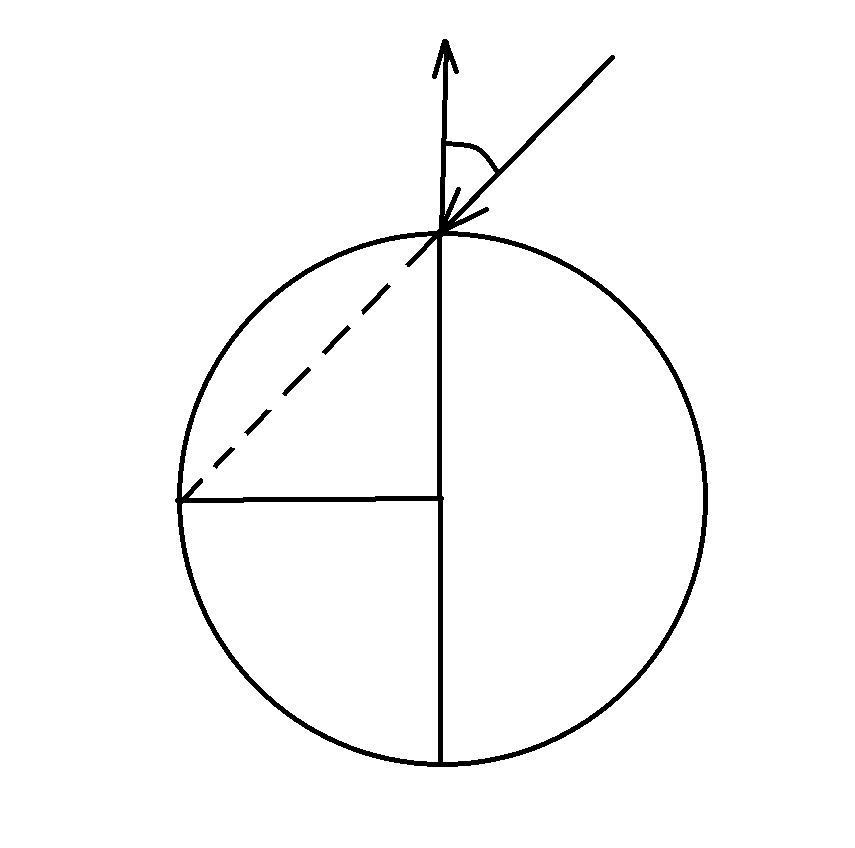
\includegraphics[scale=0.7]{11.7.png}
\caption{Задача 11.7}
\label{fig:Kick hyro}
\end{figure}

\[L_{\|} = I \omega = \frac{2\pi M R^2}{5T}\]

\[L_{\bot} = mVR\sin \varphi = \frac{mVR}{\sqrt{2}}\]

\[\alpha = \frac{L_{\bot}}{L_{\|}} = \frac{mVR}{\sqrt{2}} \cdot \frac{5T}{4\pi M R^2} = 1,27 \cdot 10^{-17} \textit{рад}\]

Можем заметить, что такое кратковременное воздействие сдвинуло Землю всего лишь на $1,27 \cdot 10^{-17}$ радиан.

Теперь же рассмотрим воздействие на гироскоп кратковременной но очень большой по модулю силы. Она вызовет временное несовпадение оси вращения и главной оси инерции и мы сможем наблюдать колебания оси (нутацию), которые будут затухать в результате трения.

\end{document}